\begin{abcliste}
\abc
\begin{center}
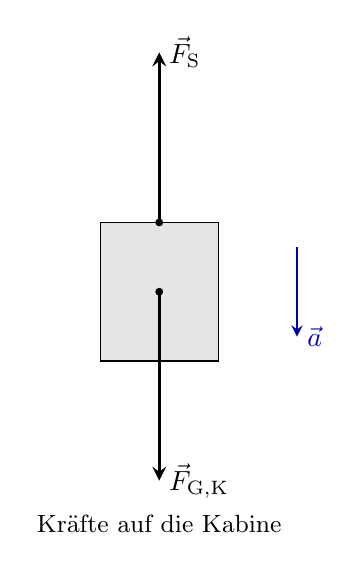
\begin{tikzpicture}[>=stealth]
 \draw[fill=gray!20] (-0.75,-0.88) rectangle (0.75,0.88);
 \draw[->, very thick] (0,0.88) -- (0,3.04);
 \fill (0,0.88) circle (0.05);
 \node[right] at (0,3.04) {$\vec F_\mathrm{S}$};
 \draw[->, very thick] (0,0) -- (0,-2.4);
 \fill (0,0) circle (0.05);
 \node[right] at (0,-2.4) {$\vec F_\mathrm{G,K}$};
 \draw[->, thick, blue!70!black] (1.75,0.57) -- (1.75,-0.57) node[right] {$\vec a$};
 \node[font=\small] at (0,-2.95) {Kräfte auf die Kabine};
\end{tikzpicture}
\hspace{1cm}
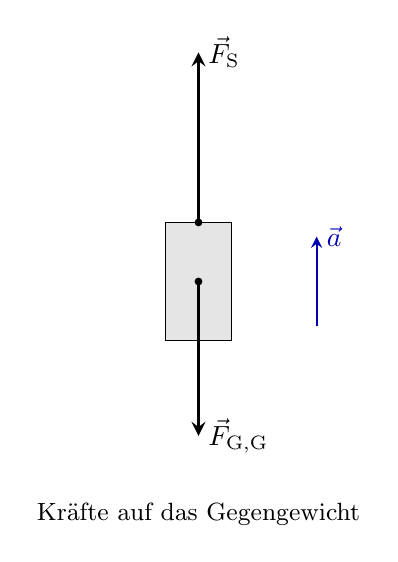
\begin{tikzpicture}[>=stealth]
 \draw[fill=gray!20] (-0.42,-0.75) rectangle (0.42,0.75);
 \draw[->, very thick] (0,0.75) -- (0,2.91);
 \fill (0,0.75) circle (0.05);
 \node[right] at (0,2.91) {$\vec F_\mathrm{S}$};
 \draw[->, very thick] (0,0) -- (0,-1.96);
 \fill (0,0) circle (0.05);
 \node[right] at (0,-1.96) {$\vec F_\mathrm{G,G}$};
 \draw[->, thick, blue!70!black] (1.5,-0.57) -- (1.5,0.57) node[right] {$\vec a$};
 \node[font=\small] at (0,-2.95) {Kräfte auf das Gegengewicht};
\end{tikzpicture}
\end{center}
Beide Bilder haben denselben Massstab.

Entlang des Seils bilden Kabine und Gegengewicht ein System: Die Differenz ihrer Gewichtskräfte beschleunigt beide Massen.
\begin{align}
 a &= \aF \\
   &= \frac{(\mK-\mG)\cdot\g}{\mK+\mG} \\
   &= \a \approx \result{\aP{0}{2}}
\end{align}
Das Gegengewicht erleichtert dem Motor die Arbeit und macht den Fall langsamer.

\abc
Das Gegengewicht allein: Es wird nach oben beschleunigt, also zieht das Seil es mit mehr als seiner Gewichtskraft.
\begin{align}
 \ssc{F}{S} - m_\mathrm{G}\,g &= m_\mathrm{G}\,a \\
 \ssc{F}{S} &= \FSF \\
   &= \mG\cdot(\g+\a) \\
   &= \FS \approx \result{\FSP{3}{2}}
\end{align}
Kontrolle mit der Kabine: $m_\mathrm{K}\,g - \ssc{F}{S} = m_\mathrm{K}\,a$.
\end{abcliste}
